\documentclass{article}
\usepackage[utf8]{inputenc}
\usepackage{textcomp}
\usepackage{graphicx}
\usepackage{float}
\usepackage{array}

% Tabelle
\usepackage{tabu}
\usepackage{caption} 
\captionsetup[table]{skip=2pt}

% Impostazioni di pagina e margini
\usepackage[a4paper, margin=2.54cm]{geometry}

% Spacing nelle liste
\usepackage{enumitem}
\setlist{topsep=2pt, itemsep=2pt, partopsep=2pt, parsep=2pt}

% Cambio di nome di contenuti Latex
\renewcommand*\contentsname{Indice}
\renewcommand{\figurename}{Figura}
\renewcommand{\tablename}{Tabella}

% Header & Footer
\usepackage{fancyhdr}
\pagestyle{fancy}
\fancyhf{}
\lhead{Progetto finale di Reti Logiche - a.a. 2018/2019}
\rhead{Motta Dennis}
\cfoot{\thepage}

% Titolo e informazioni
\title{Progetto finale di Reti Logiche}
\author{Motta Dennis - Matricola n. 865833}
\date{Anno Accademico 2018/2019}


\begin{document}

\maketitle
\tableofcontents

%%%%%%%%%%%%%%% INTRODUZIONE %%%%%%%%%%%%%%%
\pagebreak
\section{Introduzione}
Il mio obiettivo per questo progetto, oltre a creare un design funzionante in pre e post sintesi che rispetti le specifiche, è stato quello di creare un componente che arrivasse al risultato il più velocemente possibile, sfruttando quindi ogni ciclo di clock, ma senza dimenticare di scrivere codice pulito, semplice, senza ripetizioni e di facile manutenzione.\\
Queste scelte progettuali portano anche alcuni svantaggi: con un focus sulla velocità totale le caratteristiche di massima frequenza del clock e di area occupata passano in secondo piano. Non si è scelto un focus sull'area occupata in quanto la FPGA scelta ha centinaia di migliaia di Flip-Flop e LUT mentre il componente sintetizzato ne usa un numero nell'ordine delle centinaia. Anche un focus su una maggiore frequenza di clock è stato messo in secondo piano in quanto il progetto ha già un clock dato da specifica di 100ns.

\subsection{Funzionamento in sintesi}
In una breve sintesi introduttiva, si può rappresentare il funzionamento di base del componente attraverso un numero finito di step (e ciò verrà rappresentato architetturalmente attraverso una macchina a stati finiti):
\begin{enumerate}
  \item Reset; Attesa del segnale di start.
  \item Inizializzazione degli output del componente mandando la richiesta di lettura della maschera d'ingresso.
  \item Lettura dalla RAM e salvataggio in un registro della maschera di ingresso.
  \item Lettura e salvataggio della X del punto da valutare.
  \item Lettura e salvataggio della Y del punto da valutare.
  \item Lettura e salvataggio della X del 1° centroide.
  \item Lettura della Y del 1° centroide. Se il centroide va considerato per la maschera d'ingresso si calcola la distanza tra il punto da valutare e il centroide. Se questa distanza è minore della distanza minima la si salva e si sovrascrive la maschera di uscita temporanea, se essa invece è uguale alla distanza minima si pone il primo bit a '1' nella maschera di uscita temporanea.
  \item In modo equivalente 2°, 3°, 4°, 5°, 6° e 7° centroide... \addtocounter{enumi}{11}
  \item Lettura e salvataggio della X del 8° centroide.
  \item Lettura della Y del 8° centroide. Se il centroide va considerato per la maschera d'ingresso si calcola la distanza tra il punto da valutare e il centroide. Se questa distanza è minore della distanza minima la si salva e si sovrascrive la maschera di uscita temporanea, se essa invece è uguale alla distanza minima si pone l'ottavo bit a '1' nella maschera di uscita temporanea.
  \item Scrittura sulla RAM della maschera di uscita; Segnalazione di fine elaborazione usando il segnale \textit{o\_done}; Attesa del segnale di fine (\textit{i\_start} posto a '0') che ci permetterà di ritornare allo step 1 per una possibile successiva elaborazione.
\end{enumerate}

\subsection{Obiettivo velocità} \label{subsection-ob-vel}
Per raggiungere l'obiettivo della velocità si è dovuto tenere in considerazione le limitazione della RAM: a ogni ciclo di clock solo una lettura o una scrittura. La RAM quindi ha imposto un limite massimo di velocità raggiungibile. Per raggiungere questo limite si è creato un codice in cui l'elaborazione e la presentazione dei segnali di output avvenisse nello stesso ciclo di clock in cui viene fatta la lettura del dato.\\
Una volta raggiunto il limite imposto dalla RAM si sono applicate alcune ottimizzazioni per raggiungere la massima velocità per il calcolo della maschera di uscita:
\begin{enumerate}
  \item Si evita la lettura sia del valore X che del valore Y di centroidi che sono disattivati nella maschera di ingresso
  \item Viene presentato il risultato immediatamente quando i bit attivati (bit '1') nella maschera di ingresso sono in numero uguale a 0 o 1 (esempio: "00100000"). In questi casi la maschera di output è necessariamente identica alla maschera di ingresso.
  \item Si passa al centroide successivo (tenendo in considerazione l'ottimizzazione n°1) quando alla lettura del valore X del centroide si trova che la distanza sulle ascisse del centroide col punto da valutare è maggiore della distanza minima fino a quel momento trovata. (esempio: distanza minima = 4; punto da valutare X = 78; centroide X = 12; in questo caso la distanza sulle ascisse è pari a 78-12=66 che è già maggiore della distanza minima, si passa quindi al centroide successivo)
\end{enumerate}

\subsection{Obiettivo codice semplice}
Per scrivere codice semplice e "pulito" si è deciso di usare il meno possibile funzionalità algoritmiche (process), ciò per cercare di non utilizzare il linguaggio VHDL come se fosse un linguaggio di programmazione software. Il codice è quindi organizzato in diverse funzionalità, tutte inserite in un singolo modulo (entity), questa decisione puramente personale è stata presa per non complicarlo inutilmente.\\
Infine si sono create due costanti e un generic per rendere il codice facilmente espandibile a possibili modifiche:
\begin{itemize}
\item MEM\_BITS : costante che indica il numero di bit per un indirizzo di memoria. Per soddisfare la specifica di default è assegnato il valore 16.
\item CELL\_BITS : costante che indica il numero di bit in una cella di memoria che si assume equivalente al numero di centroidi da analizzare. Per soddisfare la specifica di default è assegnato il valore 8.
\item START\_ADDRESS : generic che facilita la modifica dell'indirizzo iniziale di memoria (dove è quindi salvata la maschera d'ingresso). Per soddisfare la specifica di default è assegnato il valore 0.
\end{itemize}


%%%%%%%%%%%%%%% ARCHITETTURA %%%%%%%%%%%%%%%
\pagebreak
\section{Architettura}

\subsection{Macchina a Stati Finiti}
Il funzionamento non ottimizzato del componente è stato implementato attraverso una FSM che usa come segnale di ingresso \textit{i\_start}. In realtà il passaggio agli stati successivi è dato da condizioni più complesse che permettono l'ottimizzazione.
La FSM non ottimizzata è rappresentata in figura \ref{fig:FSM}, mentre ciò che ogni stato rappresenta è spiegato più in dettaglio in tabella \ref{tab:FSM}.

\begin{figure}[H]
\centering
\caption{Macchina a Stati Finiti implementata}
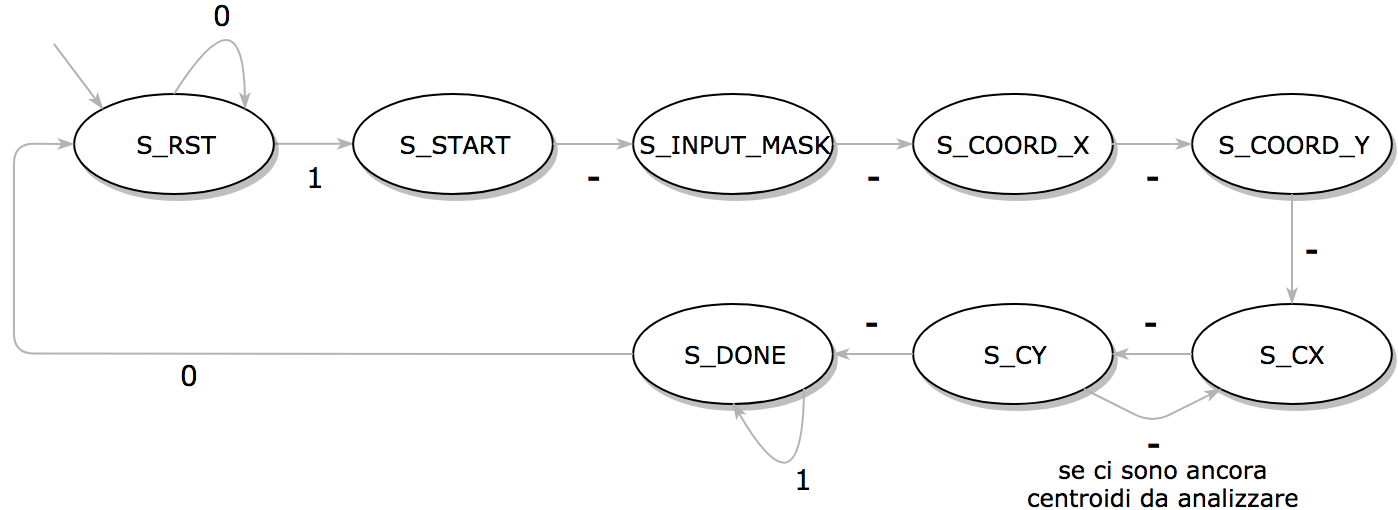
\includegraphics[width=1.0\textwidth]{FSM.png}
\label{fig:FSM}
\end{figure}

\setlength\intextsep{0mm}
\begin{table}[H]
\centering
\caption{Stati della FSM}
\begin{tabu} to 1.0\textwidth { | X[1] | X[4.0] | }
\hline
 S\_RST & Stato di partenza della FSM e stato in cui si andrà in presenza di un segnale \textit{i\_rst}. Se si riceve un segnale \textit{i\_start} si passa allo stato S\_START.\\
\hline
S\_START & Stato iniziale. In questo stato viene fornito alla RAM l'indirizzo della maschera di ingresso specificato dal generic START\_ADDRESS. \\
\hline
S\_INPUT\_MASK & Stato in cui il componente legge e salva in un registro la maschera di ingresso che gli è arrivata da memoria. \\
\hline
S\_COORD\_X & Stato in cui il componente legge e salva in un registro la X del punto da valutare che gli è arrivata da memoria. \\
\hline
S\_COORD\_Y & Stato in cui il componente legge e salva in un registro la Y del punto da valutare che gli è arrivata da memoria. \\
\hline
S\_CX & Lettura e salvataggio delle X dei centroidi. \\
\hline
S\_CY & Lettura delle Y dei centroidi. Si calcola la distanza tra il punto da valutare e il centroide, se essa è minore della distanza minima si salva questa nuova distanza e si sovrascrive la maschera di uscita temporanea, se essa invece è uguale alla distanza minima si pone il bit corrispondente a '1' nella maschera di uscita temporanea. \\
\hline
S\_DONE & Stato in cui si segnala che il risultato è stato scritto in RAM: \textit{o\_done} è portato ad '1'. Alla ricezione di \textit{i\_start} uguale a '0' si riporta la macchina in S\_RST per una possibile successiva elaborazione. \\
\hline
\end{tabu}
\label{tab:FSM}
\end{table}

\subsubsection{Ottimizzazioni effettuate}
Per arrivare al risultato nel modo più veloce possibile si sono applicate alcune ottimizzazioni già introdotte nella sezione \ref{subsection-ob-vel} a pagina \pageref{subsection-ob-vel}. Vediamo più in dettaglio gli effetti sulla FSM:
\begin{enumerate}
  \item Si evita la lettura di centroidi che sono disattivati nella maschera di ingresso, ciò significa che lo stato S\_CX verrà percorso un numero di volte pari al numero di bit attivi nella maschera di ingresso. 
  \item Alla lettura della maschera di ingresso che avviene nello stato S\_INPUT\_MASK, se si scopre che essa ha 0 o 1 bit attivati, si passa direttamente allo stato S\_DONE scrivendo il risultato nella RAM.
  \item Alla lettura della X di un qualsiasi centroide che avviene nello stato S\_CX, se si trova che la distanza sulle ascisse tra il centroide e il punto da valutare è maggiore della distanza minima fino a quel momento trovata, si passa al centroide successivo rimanendo quindi nello stato S\_CX (il centroide successivo è calcolato tenendo presente l'ottimizzazione n°1).
\end{enumerate}

\subsection{Schema funzionale}
\begin{figure}[H]
\centering
\caption{Schema funzionale del componente}
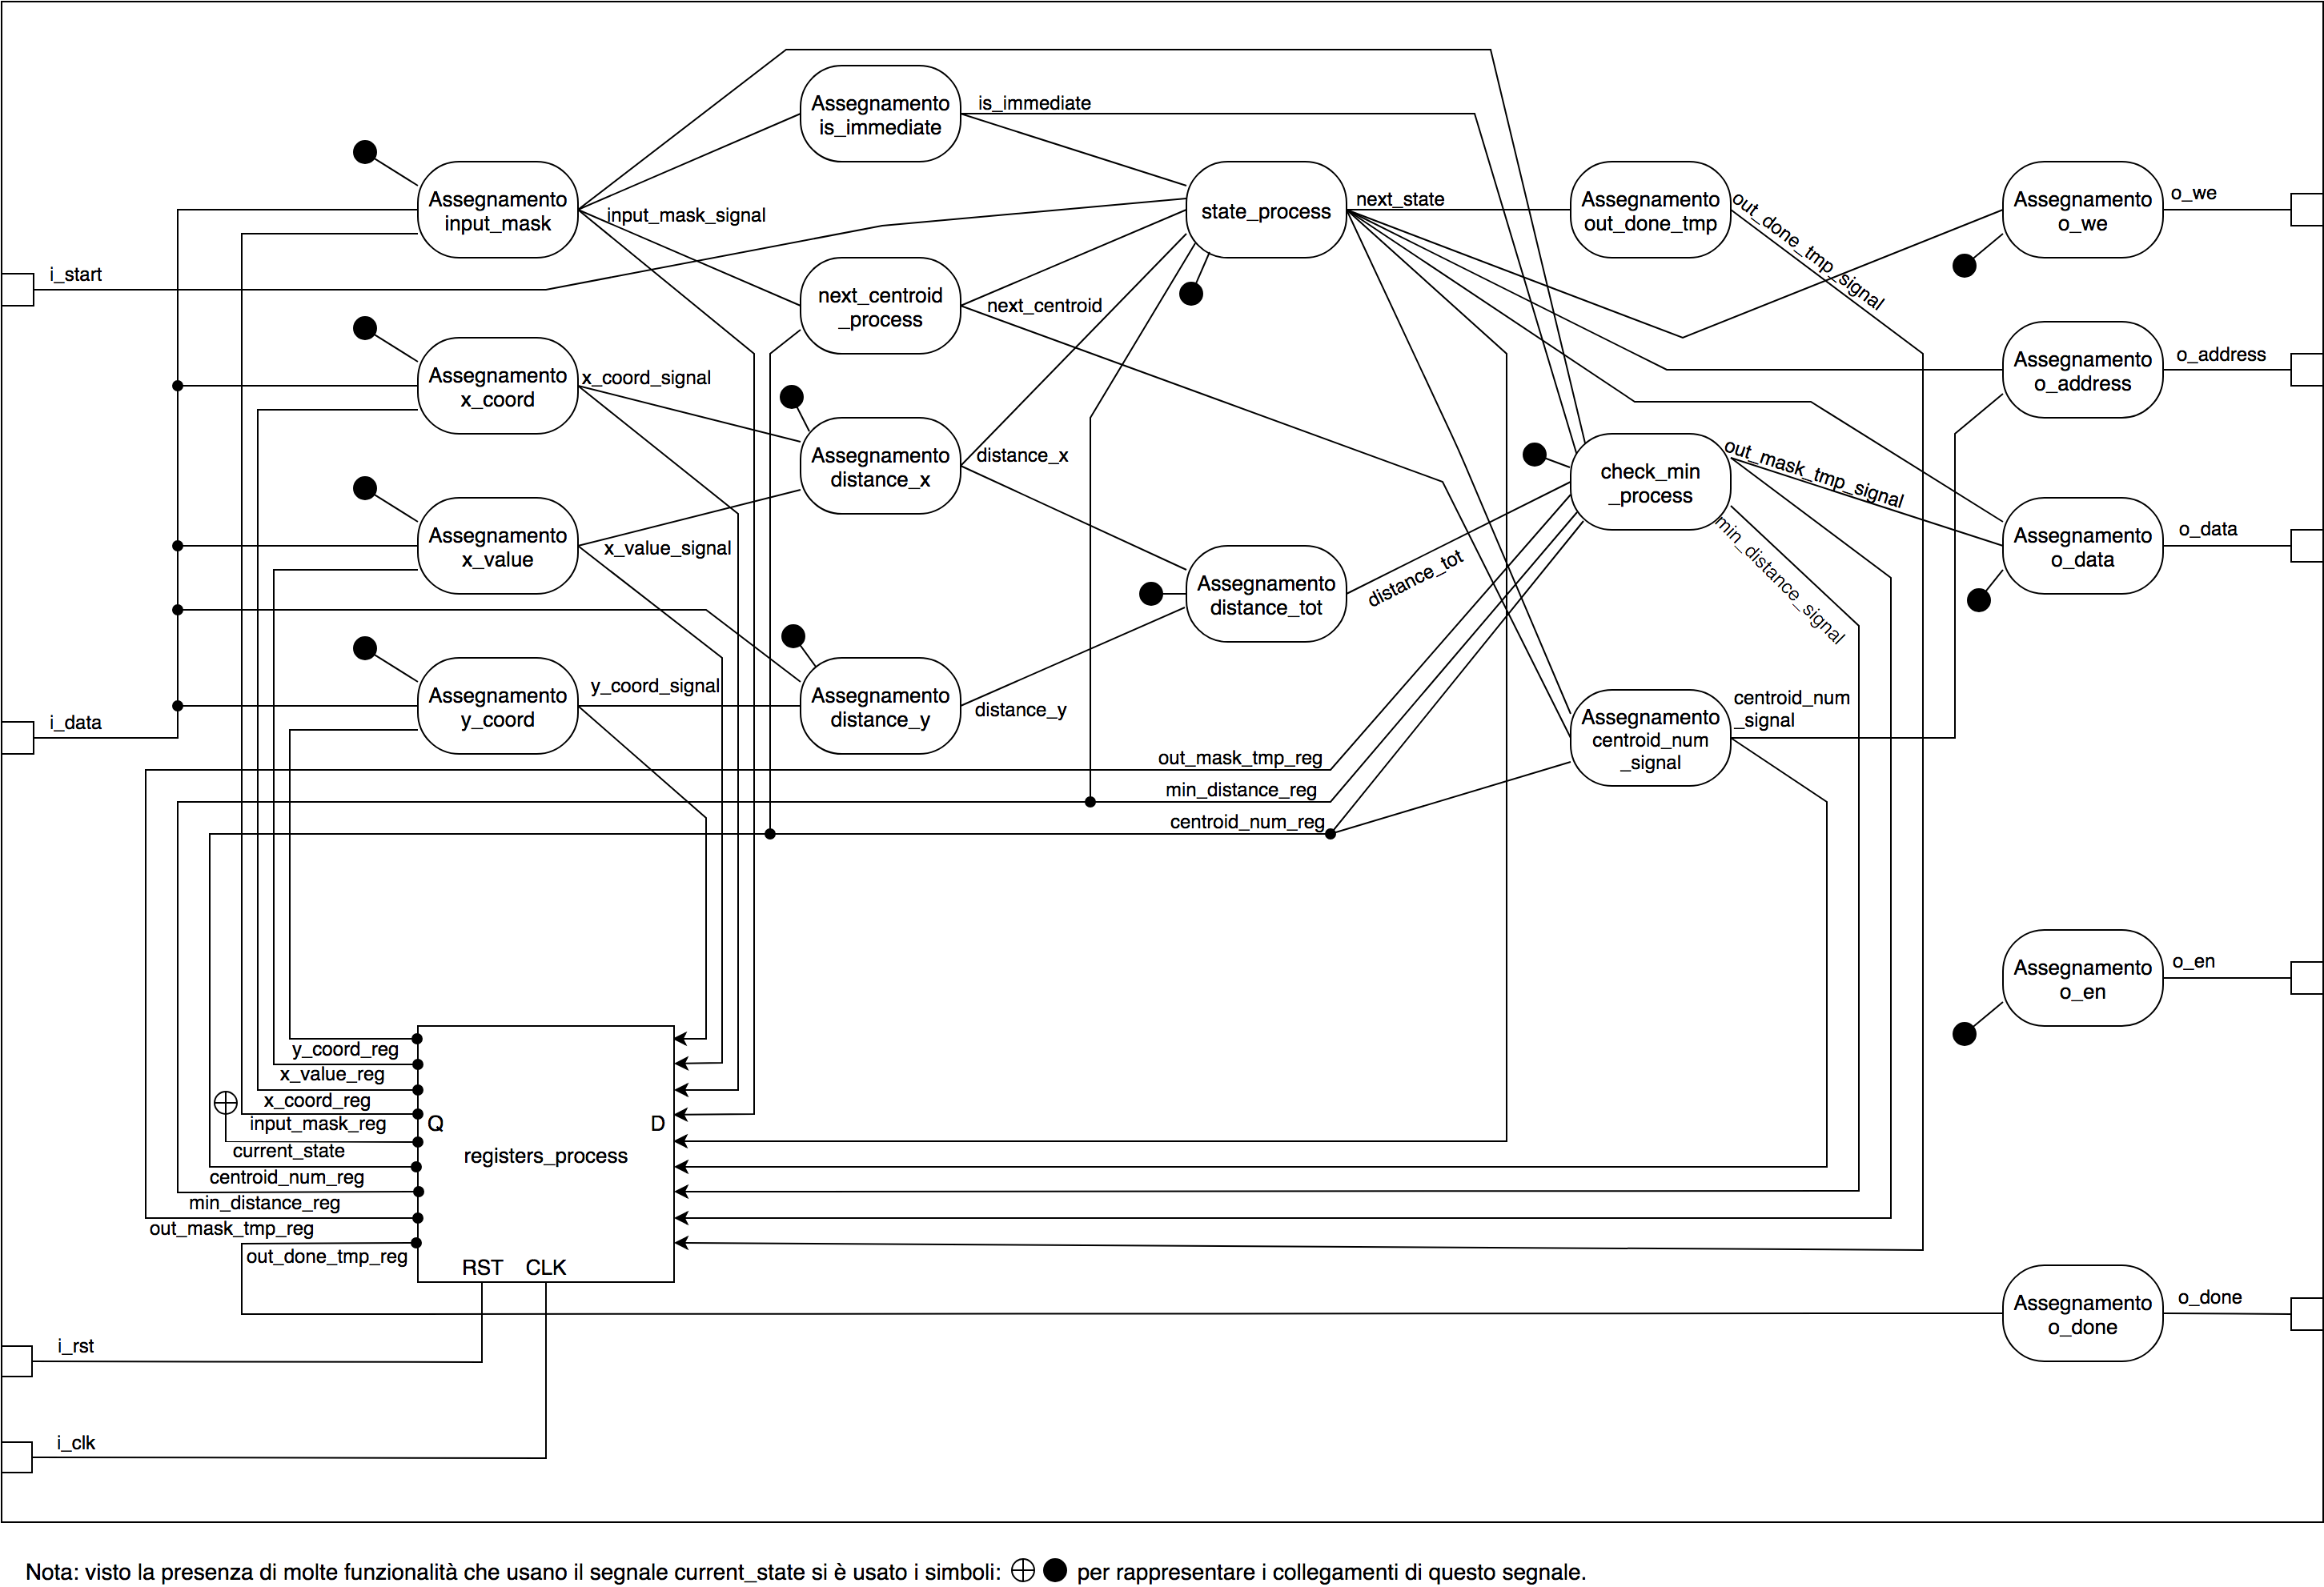
\includegraphics[width=1.0\textwidth]{Schema.png}
\label{fig:Schema}
\end{figure}
Come si può vedere in figura \ref{fig:Schema}, come architettura del componente si è usato quattro process per alcune funzionalità più complesse, tutte le altre invece sono state scritte in modo non algoritmico.
I process sono stati usati per i registri (\textit{registers\_process}), per la macchina a stati finiti (\textit{state\_process}), per trovare il prossimo stato in base alla maschera d'ingresso (\textit{next\_found\_state\_process}) e infine per controllare se il centroide in considerazione è a distanza minima (\textit{check\_min\_process}).


%%%%%%%%%%%%%%% RISULTATI SPERIMENTALI %%%%%%%%%%%%%%%
\pagebreak
\section{Risultati sperimentali}
Presentazione dei test bench...

\subsection{Test Bench 1}
Cosa fa...

\subsection{Test Bench 2}
Cosa fa...


\section{Conclusioni}
Conclusione...

\end{document}
